\documentclass[titlepage, 12pt]{article}

\usepackage[margin=1.25in]{geometry}
\usepackage{fancyhdr}
\setlength\headheight{15pt}

\pagestyle{fancy}

\usepackage{xcolor}

\usepackage{graphicx}

\usepackage{float}
\restylefloat{table}

\usepackage{bookmark}
\bookmarksetup{
  open,
  depth=2
}

\newenvironment{packed_itemize}{
  \vspace{-\topsep}
  \begin{itemize}
    \setlength{\itemsep}{1pt}
    \setlength{\parskip}{0pt}
    \setlength{\parsep}{0pt}
  }{\end{itemize}}

\newcommand{\authorName}{Nicola Pfister \& Jonas Meise}

\lhead{WaaS - WebE FFHS}
\rhead{\authorName}

\author{\authorName}
\title{WaaS - Documentation \\ \medskip \large WebE - FFHS}

\begin{document}

\maketitle

\pagebreak

\renewcommand{\contentsname}{Table of Contents}

\tableofcontents

\pagebreak

\section{Introduction}

This is the documentation of the project "Web-scraper as a Service" or WaaS for short, which was done as part of the module Web Engineering at the FFHS. The goal of the project is to create a concept and implement a web application which fulfills at least the following criteria:

\begin{itemize}
  \item Basic user authentication (register, login/logout, delete and update user)
  \item Public and dynamic/user specific content
  \item Persist user data (in database or file)
  \item Basic validation and error handling
  \item Support for sessions and cookies
\end{itemize}

The technologies for the project were not predefined, so we decided to use .NET Core for the web application and AngularJS for the front end due to personal preferences.

\pagebreak

\section{Requirements Engineering\label{sectionRequirementsEngineering}}

This chapter contains purpose and context of the web application WaaS as well as the functional and non-functional requirements.

\begin{itemize}
  \item \textbf{Name of the application:} WaaS
  \item \textbf{Purpose:} WaaS is a web application that allows it's users to scrape urls with specified search patterns and notifies them as it finds the pattern.
  \item \textbf{Names:} Nicola Pfister, Jonas Meise
\end{itemize}

\subsection{Purpose \& Context}

WaaS is a service, that allows users to keep track of news on their favourite websites, by giving them the possibility to create "Scrapes". A Scrape is defined with a URL, a search pattern and an E-Mail address. WaaS will regularly check those URLs for the given search patterns and notifies the users via their E-Mail address when it finds the pattern it was searching for.
\medskip \\
The following graphic visualizes the context of the app with it's use cases.

\begin{figure}[H]
  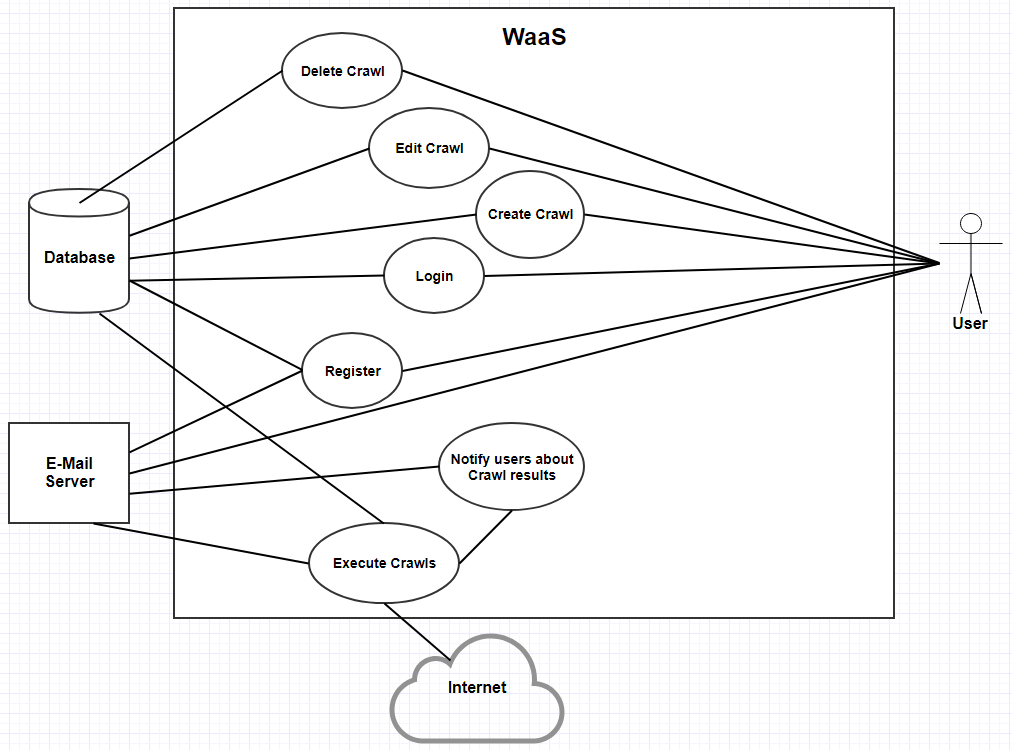
\includegraphics[width=0.95\linewidth]{UseCaseDiagram.PNG}
  \caption{Use Case Diagram}
  \label{fig:useCaseDiagram}
\end{figure}

\subsection{Functional Requirements}

The following chapter contains the functional requirements for WaaS.

\subsubsection{Target Group}

The target group of WaaS are mainly people that are regularly checking websites for news. That concludes people of all ages who understand what a web scraper is. It can also be used from people who want to check wether or not the new episode of their favourite tv series is already online. All of those people are generally expected to have some basic skills in the field of IT or are at least interested in it.

\subsubsection{{Use Cases}}

\begin{table}[H]
  \begin{center}

    \begin{tabular}{p{4cm}|p{10cm}}
      \textbf{UST-1}   & \textbf{Register}                                                                                            \\
      \hline
      Goal             & A user registers a user account for WaaS.                                                                    \\
      \hline
      Actors           & Eventual user of WaaS                                                                                        \\
      \hline
      Precondition     & The user owns a valid E-Mail address that is not yet used for an existing user account                        \\
      \hline
      Trigger          & Click on the button: "Register"                                                                              \\
      \hline
      Main path        &
      \begin{packed_itemize}
        \item [1] The user clicks the button: "SignUp".
        \item [2] The user enters his credentials into the register form (E-Mail address, and password).
        \item [3] The user clicks on: "Register".
        \item [4] WaaS creates a user account entry in the database.
        \item [5] The user gets redirected to the Login Page.
      \end{packed_itemize}                                                                                                       \\
      \hline
      Alternative path &
      \begin{packed_itemize}
        \item [1a] The user enters a invalid input data.
        \item [2a] A validation error message shows up.
      \end{packed_itemize}                                                                                                       \\
      \hline
      Postcondition    & A new user account was created in the database with the credentials the user entered into the register form. \\
    \end{tabular}

    \caption{UST-1}
    \label{table:UST-1}

  \end{center}
\end{table}

\begin{table}[H]
  \begin{center}

    \begin{tabular}{p{4cm}|p{10cm}}
      \textbf{UST-2}   & \textbf{Login}                                                 \\
      \hline
      Goal             & A user logs in with an existing user account.                  \\
      \hline
      Actors           & registered users                                               \\
      \hline
      Precondition     & UST-\ref{table:UST-1}                                          \\
      \hline
      Trigger          & Click on the button: "LogIn"                                   \\
      \hline
      Main path        &
      \begin{packed_itemize}
        \item [1] The user enters a valid E-Mail address an password into the login form.
        \item [2] The user clicks on the button: "LogIn".
      \end{packed_itemize}                                                         \\
      \hline
      Alternative path &
      \begin{packed_itemize}
        \item [1a] The user enters a invalid input data.
        \item [2a] A validation error message shows up.
      \end{packed_itemize}                                                         \\
      \hline
      Postcondition    & The user is now logged in and is situated on the overview page \\
    \end{tabular}

    \caption{UST-2}
    \label{table:UST-2}

  \end{center}
\end{table}

\begin{table}[H]
  \begin{center}

    \begin{tabular}{p{4cm}|p{10cm}}
      \textbf{UST-3}   & \textbf{Create Scrape}                                                                                             \\
      \hline
      Goal             & A user creates a new scrape.                                                                                       \\
      \hline
      Actors           & logged in users                                                                                                    \\
      \hline
      Precondition     & UST-\ref{table:UST-1} \& UST-\ref{table:UST-2}                                                                     \\
      \hline
      Trigger          & Click on the button: "+"                                                                                           \\
      \hline
      Main path        &
      \begin{packed_itemize}
        \item [1] The user enters a URL into the New Scrape form.
        \item [2] The form shows if the entered URL is valid.
        \item [3] The user enters a Scrape pattern into the New Scrape form.
        \item [4] The user clicks on the button: "Save".
      \end{packed_itemize}                                                                                                             \\
      \hline
      Alternative path &
      \begin{packed_itemize}
        \item [1a] The user clicks the button "Cancel".
      \end{packed_itemize}                                                                                                             \\
      \hline
      Postcondition    & The newly created scrape is persisted in the database \& The new scrape gets displayed on the users overview page. \\
    \end{tabular}

    \caption{UST-3}
    \label{table:UST-3}

  \end{center}
\end{table}

\begin{table}[H]
  \begin{center}

    \begin{tabular}{p{4cm}|p{10cm}}
      \textbf{UST-4}   & \textbf{Delete Scrape}                                                                                           \\
      \hline
      Goal             & A user deletes an existing scrape.                                                                               \\
      \hline
      Actors           & logged in user                                                                                                   \\
      \hline
      Precondition     & UST-\ref{table:UST-3}                                                                                            \\
      \hline
      Trigger          & Click on the delete scrape button.                                                                               \\
      \hline
      Main path        &

      \begin{packed_itemize}
        \item [1] The user clicks on the delete button of the scrape he wishes to remove.
        \item [2] A confirmation dialogue is shown.
        \item [3] The user clicks the "Delete" button.
        \item [4] The scrape gets deleted from the database.
      \end{packed_itemize}                                                                                                          \\
      \hline
      Alternative path &
      \begin{packed_itemize}
        \item [3a] The user clicks the button "Cancel".
        \item [4a] The confirmation dialogue closes.
      \end{packed_itemize}                                                                                                          \\
      \hline
      Postcondition    & The scrape is deleted from the database \& The scrape does not get displayed on the users overview page anymore. \\
    \end{tabular}
    \vspace{-2mm}
    \caption{UST-4}
    \label{table:UST-4}

  \end{center}
\end{table}

\begin{table}[H]
  \begin{center}

    \begin{tabular}{p{4cm}|p{10cm}}
      \textbf{UST-5}   & \textbf{Edit Scrape}                                    \\
      \hline
      Goal             & A user edits an existing scrape.                        \\
      \hline
      Actors           & logged in user                                          \\
      \hline
      Precondition     & UST-\ref{table:UST-3}                                   \\
      \hline
      Trigger          & Click on the edit scrape button.                        \\
      \hline
      Main path        &
      \begin{packed_itemize}
        \item [1] The user clicks on the edit button of the Scrape he wishes to edit.
        \item [2] The Edit Scrape form is shown.
        \item [3] The user changes the Scrape's URL.
        \item [4] The form shows if the entered URL is valid.
        \item [5] The user clicks "Save".
        \item [6] The changes get persisted in the database.
      \end{packed_itemize}                                                 \\
      \hline
      Alternative path &
      \begin{packed_itemize}
        \item [2a] The user clicks the button "Cancel".
        \item [3a] The Edit Scrape form closes.
      \end{packed_itemize}                                                 \\
      \hline
      Postcondition    & The updated Scrape gets displayed on the overview page. \\
    \end{tabular}

    \vspace{-2mm}
    \caption{UST-5}
    \label{table:UST-5}

  \end{center}
\end{table}

\begin{table}[H]
  \begin{center}

    \begin{tabular}{p{4cm}|p{10cm}}
      \textbf{UST-6}                & \textbf{Receive and Dismiss Notification}                    \\
      \hline
      Goal                          & A user gets notified about a Scrape having been triggered.   \\
      \hline
      Actors                        & user                                                         \\
      \hline
      Precondition                  & UST-\ref{table:UST-3}                                        \\
      \hline
      Trigger                       & WaaS found defined Scrape pattern on Scrape URL.             \\
      \hline
      Main path                     &
      \begin{packed_itemize}
        \item [1] The user receives an E-Mail notifying him about the triggered Scrape.
        \item [2] The user clicks on the link in the E-Mail.
        \item [3] The notification gets dismissed by the system.
        \item [4] The user gets redirected to the URL of the Scrape.
      \end{packed_itemize}                                                                   \\
      \hline
      Alternate path:                                                                              \\
      Notification Tray             &
      \begin{packed_itemize}
        \item [1a] The user logs in to WaaS.
        \item [1b] The user opens the notification tray.
        \item [2a] The user clicks on the notification in the tray
      \end{packed_itemize}                                                                   \\
      \hline
      Alternate path:                                                                              \\
      Notification Tray Dismiss All &
      \begin{packed_itemize}
        \item [1a] The user logs in to WaaS.
        \item [1b] The user opens the notification tray.
        \item [2a] The user dismisses all notifications.
        \item [3a] All previously unread notifications get marked read.
      \end{packed_itemize}                                                                   \\
      \hline
      Postcondition                 & The user has been notified about his scrape being triggered. \\
    \end{tabular}

    \vspace{-2mm}
    \caption{UST-6}
    \label{table:UST-6}

  \end{center}
\end{table}

\begin{table}[H]
  \begin{center}

    \begin{tabular}{p{4cm}|p{10cm}}
      \textbf{UST-7} & \textbf{Show Scrape History}                      \\
      \hline
      Goal           & A user can see all past triggers of a Scrape.     \\
      \hline
      Actors         & logged in user                                    \\
      \hline
      Precondition   & UST-\ref{table:UST-3}                             \\
      \hline
      Trigger        & User opens Scrape details.                        \\
      \hline
      Main path      &
      \begin{packed_itemize}
        \item [1] The opens the Scrape details.
        \item [2] Details include an overview of past triggers for the Scrape.
      \end{packed_itemize}                                         \\
      \hline
      Postcondition  & The user has gotten information about his Scrape. \\
    \end{tabular}

    \vspace{-2mm}
    \caption{UST-7}
    \label{table:UST-7}

  \end{center}
\end{table}

\subsection{Non-functional Requirements}

\begin{enumerate}
  \item \textbf{Performance}
        \begin{enumerate}
          \item For user interactions, the application should respond 99\% of the requests in 2 seconds.
          \item The application should score at least 40 points of performance in Google Chromes inbuilt Lighthouse audit up to a number of 500 concurrent users.
        \end{enumerate}
        Those performance related requirements will be evaluated using Performance Testing and Monitoring of the application.
  \item \textbf{Usability}
        \begin{enumerate}
          \item If the application experiences any kind of error or delay, users should be made aware of this.
          \item When a website that is subject to a Scrape changes to contain the looked for pattern, users should receive a notification within an hour.
        \end{enumerate}
        The usability requirements will be evaluated using automated Testing.
  \item \textbf{Other non-functional requirements}
        \begin{enumerate}
          \item The application should be implemented according to best practices and should therefore score 100 points in the best practices section of the Lighthouse audit.
          \item The application should have a responsive design, so it will be easy to use on a variety of devices with different screen sizes.
          \item Horizontal scalability is too big of a task to be realized in the given time frame and is therefore outside of the scope of this project. If horizontal scalability were to be achieved, a cloud database service could possibly be used to overcome the issue of relational database scaling. Since EF Core has a DB Provider for Azure Cosmos SQL API in preview, the implementation of it could be more or less of a drop-in replacement. Of course, this solution isn't currently viable for production environments and if another approach is to be used, the application's data access layer would have to be redesigned accordingly.\\
          Due to the use of SignalR which creates WebSocket based connections to the client application, there might be more issues in regards to those connections and load balancing. Azure provides a SignalR Service which might come in handy for this.\\
          Those issues are the two most obvious ones which also have a possible solution through cloud services but it is very well possible, that other issues arise in horizontally scaled WaaS environments, which we did not think of at the time of writing this document. 
          
        \end{enumerate}
\end{enumerate}

\section{GUI and Navigation Design}
\subsection{Navigation Model}

The following diagram depicts principal states and possible user interactions to navigate between them.

\begin{figure}[H]
  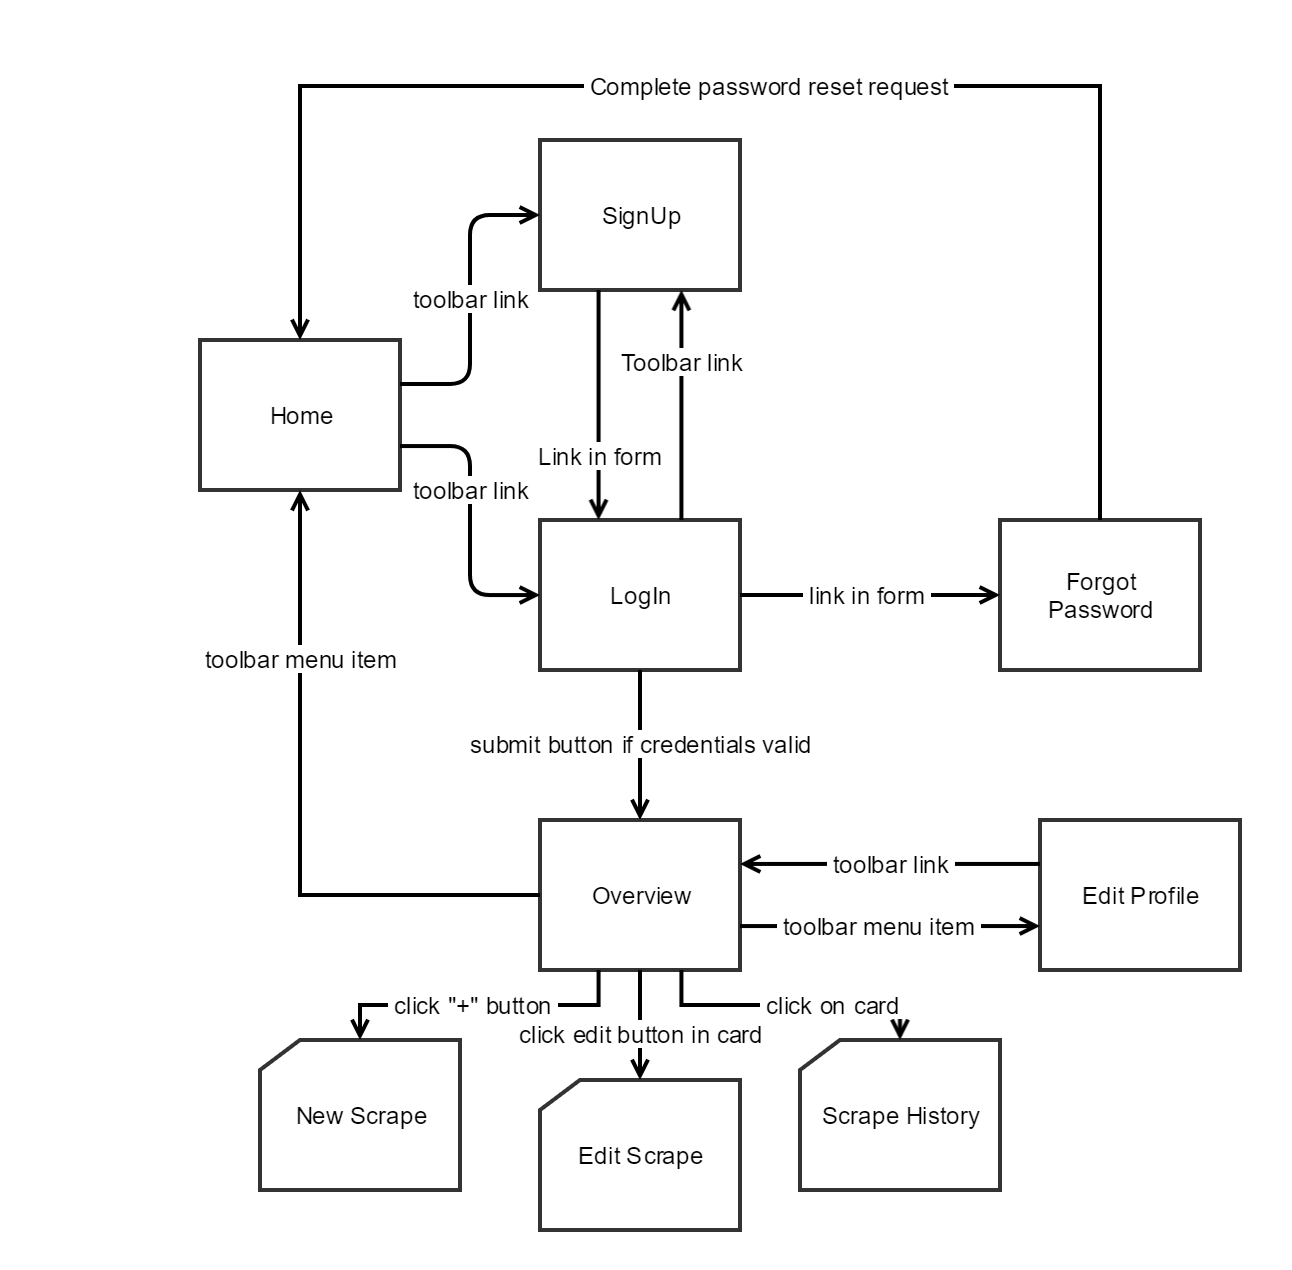
\includegraphics[width=0.95\linewidth]{navigationmodel_waas.png}
  \caption{Navigation Model}
  \label{fig:navigationModel}
\end{figure}

The boxes represent states and the arrows the means to transition from one state to another. The boxes with a missing corner represent a modal and the arrows leading up to the modals aren't state transitions since the modals don't
represent a complete state but a GUI element within their parent state. The modal blocks other interactions until it is dismissed, either through cancelling it or following through on its action. \\
The user enters the page on "Home" and needs to log in to get to the main state called "Overview". From there, all other interactions to manage Scrapes are possible. In other words, "Overview" acts as a dashboard showing all principal functionality of the application.

\subsubsection{Potential sources of errors}
The following issues may arise from the navigation.

\paragraph{User doesn't want to register}
It is possible, that a user wants to see how WaaS works, without registering beforehand.
This is not possible in the navigation model since a user needs to be logged in to use WaaS. Since it is possible for users to delete their accounts it is a minor issue though.

\paragraph{User gets lost in a branch state}
A user could get lost in a state because he doesn't see, how to leave it. Usually, a user will then use the browsers back button, so it's important to either make sure it works or to offer the user an obvious alternative back action.

\paragraph{User may not know that a click on a card shows the scrape history}
It may not be intuitive for some users to click on a card in order to display the history of a scrape. If this turns out to be a problem it could be solved by adding a button for the history.

\subsubsection{Automation in Navigation Design}

Once a navigation design was created, it can be useful to analyze it in order to find potential errors and bad design choices. For a small application where the navigation design is not that complex this can easily be achieved by hand. For more complex navigation models this may be difficult to do \cite{mSharonHurleyHall2019}. Therefore a variety of tools can be used to automate this process. One possible choice is Google Analytics. If there already is an existing website or an HTML prototype google analytics can visualize user flows and direct you to potential problems in the navigational design as described in this article \cite{mAndyCrestodina2018}.

Since WaaS is a rather small and simple application we found it unnecessary to do automated analytics of our navigation design.

\subsection{HTML Prototype}
To visualize the navigation model, a HTML Prototype was created and is available either in the adjacent documents to this documentation or through the GitHub Page on \url{https://nipfi.github.io/WaaSDoc/HTML%20Prototype/index.html}.

\section{Software Architecture}
This chapter is about the planned architectural strucutre of WaaS. The goal is to visualize some parts of the architecture for a better understanding of how WaaS is composed.

\subsection{Class Diagram}
The class diagram shows a visual representation of the class structure of WaaS. It is meant to show a basic overview and there may be some deviations from the actual implementation. Due to the size of the class diagram it is not included in this PDF file. It can be found as attachment with the name "ClassDiagram.svg".

\subsection{Sequence Diagram}
The following figure \ref{fig:sequenceDiagram} shows the procedure of a login sequence for WaaS.

\begin{figure}[H]
  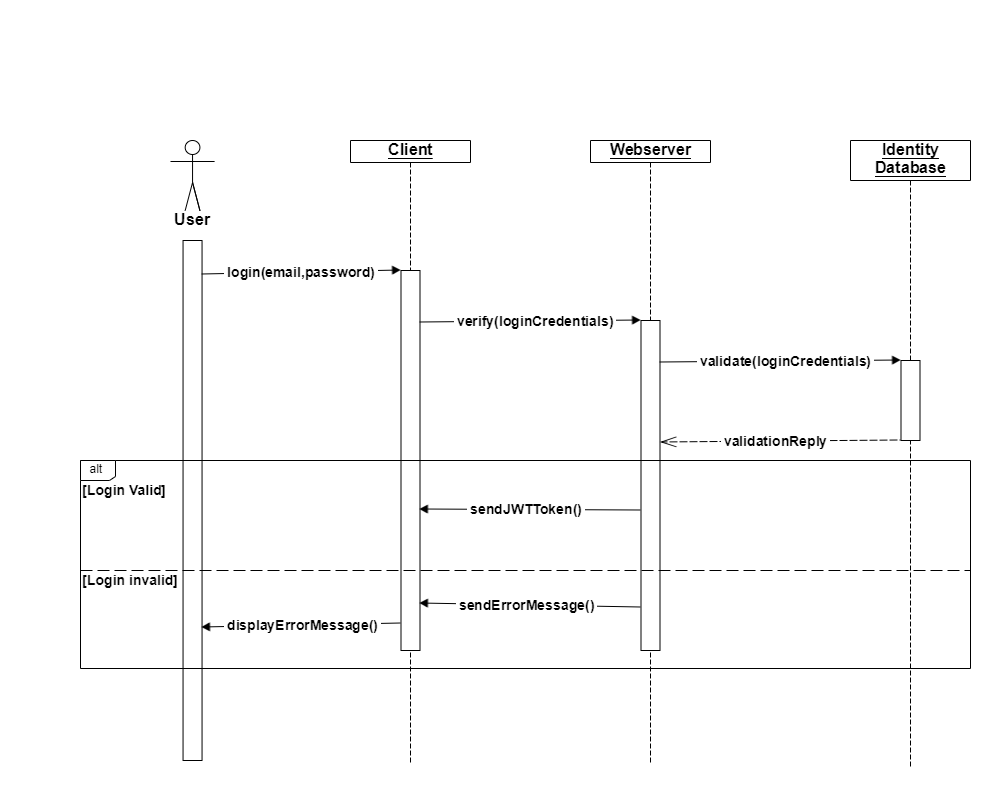
\includegraphics[width=0.95\linewidth]{SequenceDiagram.png}
  \caption{Sequence Diagram}
  \label{fig:sequenceDiagram}
\end{figure}

\subsection{Deployment Diagram}
The deployment diagram shows the environment of the Deployment process for the application WaaS. Both the Web API and the Angular Application are hosted in the azure cloud as seen in \ref{fig:deploymentDiagram}. The angular application will on request be served to the client and will be executed from there.

\begin{figure}[H]
  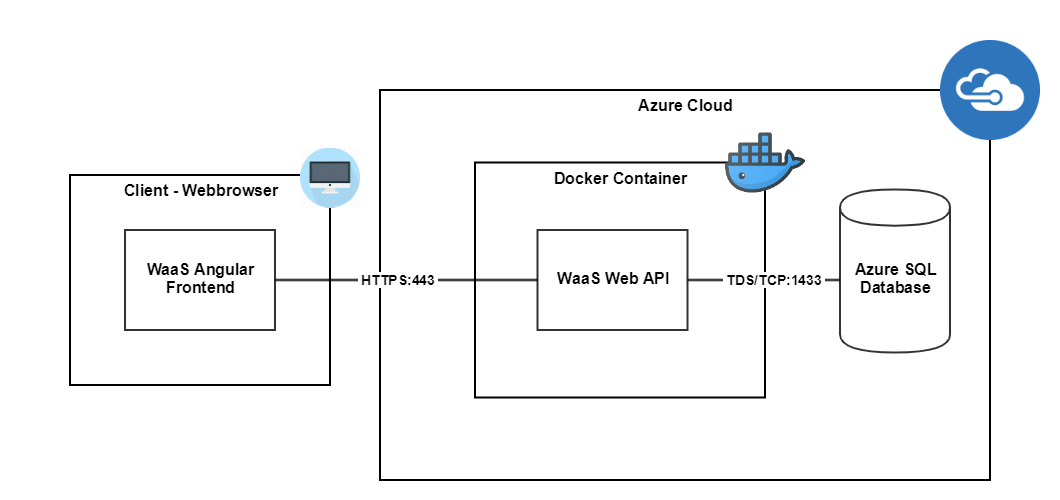
\includegraphics[width=0.95\linewidth]{DeploymentDiagram.png}
  \caption{Deployment Diagram}
  \label{fig:deploymentDiagram}
\end{figure}

\pagebreak

\section{Used technologies and frameworks}

\subsection{Front End}

\paragraph{Angular}
The front end is implemented using Angular because its dynamic nature makes it ideal for handling user interaction with a RESTful web service.
Through its architecture it promotes a clean style of coding and its reliance on TypeScript makes Front End Code much more understandable for developers with a background in object oriented programming paradigms.
Furthermore, it has a great spread in enterprise applications and because of this also a healthy developer community. \\
Angular offers most features needed for WaaS by itself, therefore no further frameworks are required. Some components and functionality may be added through 3rd party dependencies though.

We chose this technology for the front end because angular is a popular framework that we are keen on learning and using. An alternative to Angular which is also widely used is called React. We decided to go with Angular instead of React mainly because we know it better. Furthermore Angular has dependency injection and uses typescript by default, which are two aspects we like about Angular.

\subsection{Back End}

\paragraph{.NET Core}
As a relatively young part of the .NET landscape, .NET Core improves on many shortcomings of .NET Framework. Not only is it open-source, it also runs cross-platform and is generally less demanding in resources, which makes it more suited for deployments in cloud services, containerized or not.

The reason we chose the .NET environment for our Back-end is that we are used to working with it and want to get to know it better. It is commonly used by many developers and counts as one of the top technologies looked for in the industry of software development.

\subparagraph{ASP.NET Core}
ASP.NET Core is the .NET Core equivalent of the ASP.NET web application framework and provides powerful yet simple to use methods for implementing REST APIs. It practically is built-in to any
.NET Core web application project which makes it an easy choice.

\subparagraph{Entity Framework Core}
EF Core is the default O/R mapper for .NET Core projects. It offers connectors for almost any relevant relational database technology and makes it relatively easy to handle database modelling tasks
while allowing for the data model to change in a safe way through it's code-first migrations feature. It's an ideal technology for smaller web application projects.

\subparagraph{ASP.NET Core Identity}
WaaS uses ASP.NET Core Identity because in many cases it's a better choice for security to rely on a well-maintained framework rather than badly implementing a custom authentication and authorization mechanism and
since it's quite a basic requirement for many web applications, we believe it to be a better approach to consolidate efforts to promote web application security. ASP.NET Core Identity integrates very well with the other
frameworks used in this back end dependency constellation.

Nowadays it often is a wise idea to use an existing framework to handle identity management. Implementing this by yourself can lead to security flaws and one has to put a lot of work in it to achieve a secure system. That is why we decided to use ASP.NET Core Identity as our technology for identity management. An example for an alternative would be firebase auth. We did not further research alternatives since .NET Core Identity is well integrated to the .NET environment and works very well along with a ASP.NET Web API and it could be integrated with third party OAuth providers like Google or GitHub.

\subsection{Deployment}

\paragraph{Docker}
By using Docker, WaaS can be deployed in virtually any environment from a simple docker host to a more complex orchestrated container platform with relative ease.
The complexity of managing software dependencies in a restricted server environment is completely eliminated which is advantageous
even though the build process for a docker image can be tedious to maintain.

WaaS is configured to run inside a Docker container. That container contains the Web API (back-end) and Angular App (front-end). During the deployment process this docker container gets pushed to the azure container registry and will then run in the azure cloud. A visual representation of the deployed application state of WaaS can be seen in figure \ref{fig:deploymentDiagram}.

\pagebreak

\section {Usability testing methodology}
Even though there is no formal usability testing planned at the moment, WaaS should offer a good amount of user-friendliness.
If possible, users should be offered help in the form of visual guides where necessary.
Furthermore, users should be able to provide feedback for example in the form of GitHub issues or a simple E-Mail, in order to record and implement the requirements of the actual users of WaaS.
The Usability of WaaS could be evaluated by a simplified usability test with the help of friends and family.
There is also the possibility to use an Automated Expert Review for the purpose of a quick and low-cost usability review.

Lastly, A/B tests could be used to evaluate specific changes in the application which is possible due to the containerized deployment strategy allowing to have two slightly different
instances of an application up and running or to replace one version with another in a relatively easy way. An example for a possible A/B Test would be the actions a user can do with ScrapeJobs ("Show History","Edit","Delete","Toggle Enabled"). The way the actions are currently implemented is via icons on each ScrapeJob card as shown in \ref{fig:scrapeJobCard}.

\begin{figure}[H]
  \centering
  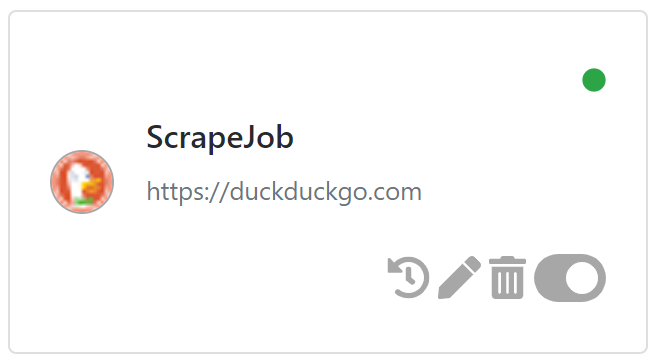
\includegraphics[width=0.5\linewidth]{scrapeJobCard.png}
  \caption{Scrape Job Card}
  \label{fig:scrapeJobCard}
\end{figure}

One other possible way to implement those actions would be as a a menu bar on top of the page with the possibility to select ScrapeJobs. This would have the advantage that for the actions "Toggle Enabled" and "Delete" you could select multiple ScrapeJobs at once.
Our hypothesis is that the icons on the ScrapeJob card are more intuitive to the user. Also it would eventually lead to a smaller error rate due to the possibility that the menu bar could lead users to think that they can also edit multiple ScrapeJobs at once.
With the help of A/B testing we could find out if our hypothesis is correct.

\pagebreak

\section{Development strategy}

As model for the development process we used a tailored version of Scrum. The tailored version of Scrum defines an iterative and agile approach for software development.

Due to the two week submission cycle of the project we used a duration of two weeks for each sprint. The sprint backlog of each cycle consists of the tasks that were predefined by the submissions. To track those backlog work items we used GitHub issues and defined milestones for the sprints. We further separated User Stories into small packages and used a Kanban board (figure \ref{fig:kanbanBoard}) in Azure DevOps to be able to work together more efficiently. The kanban board consists of the rows "To do", "In progress", "Testing" and "Done". Once one of us implemented a task and had moved it to Testing the other one reviewed it and did some manual testing. Through the kanban board we always had a good overview of the development progress. 

\begin{figure}[H]
  \centering
  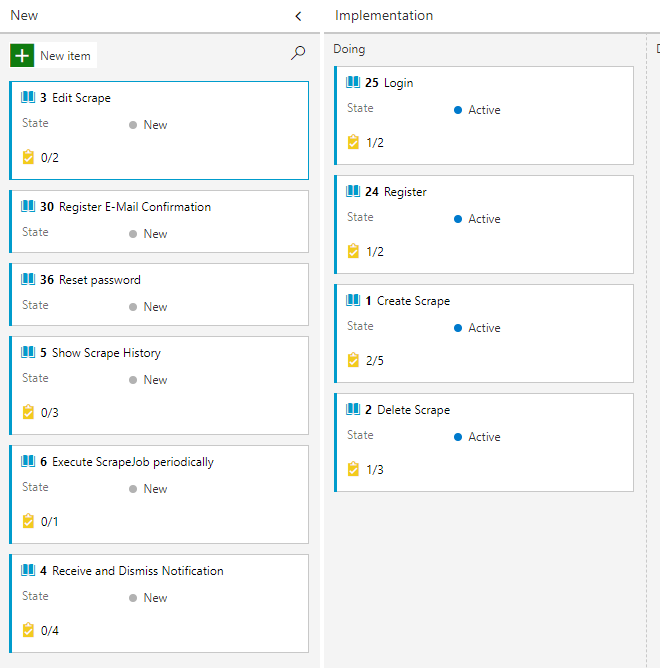
\includegraphics[width=0.65\linewidth]{KanbanBoard.png}
  \caption{Kanban Board}
  \label{fig:kanbanBoard}
\end{figure}

Since we used a tailored version of Scrum we did not do any daily Scrum meetings and had no sprint retrospective. This would not have been easily achievable due to different work times and work locations. Also we did not have a traditional Scrum management hierarchy with Scrum master and product manager due to our team size being limited to two people.

\section{Security Analysis}

In the scope of the project we analysed security aspects of WaaS. Specifically we focused on google hacking. Most of the methods described in \cite{mJohnnyLong2005} should be prevented by using third party libraries for features containing security measures. Given that we only use third party libraries of developers we can trust. Concerning google hacking there are two potential vulnerabilities we took a closer look at. We discuss them in the following sections.

\subsection{Open Source}
\label{sec:opensource}

WaaS' source code is licensed under the open source license AGPL 3.0 and can be found publicly on GitHub under \url{https://github.com/NiPfi/WaaS}. While a principle of open source software is that it can be reviewed and tested by other people this may also be a security risk. If there are any overlooked security flaws to be found in our code they can be discovered by anyone. It is then up to those people to decide if they contact us about the flaw or if they plan to do malicious actions with that information.


One way to prevent this potential security flaw would be to make our project closed source. We don't want to do so because we are supporters of open source software and we accept the risks that come with it. Also we believe that this flaw will possibly be balanced out by helping members of the community that would point out flaws in the code.


\subsection{Third party libraries}

Through advanced google searches and the usage of it's search operators it is possible to search for websites that use specific libraries. For example the npm package-lock file can be found in the source repository of our project. Therefor attackers could try to look for dependencies with known vulnerabilities and try to use those vulnerabilities to attack a hosted instance of WaaS. As our project is open source (as described in \ref{sec:opensource}) the dependencies of our projects can easily be looked up.

To minimise the risk of this security flaw we can regularly update the libraries that we use and check for known vulnerabilities ourselves. That way we can prevent security flaws of those libraries being integrated into our software.

\subsection{OWASP}

Further analysis of security aspects for this project was done concerning the OWASP Top Ten Project (\cite{mOWASPTopTen}). Due to the scope of the project this analysis is not documented here.

\section{Conclusion}

The last chapter covers our Lessons Learned and what we plan to do with WaaS in the future.

\subsection{Lessons Learned}
\label{section:LessonsLearned}

During this project we acquired many new skills. We got to explore new technologies and methods in the field of software development. Angular for example is a widely used and popular front-end technology and is often seen in combination with a REST API back-end such as an ASP.NET web service.
Further we were able to gain experience with Azure DevOps by implementing a CI/CD pipeline for our project.


While we started implementing WaaS we also noticed some of the difficulties that occur in a web development project. Even though we are a small team consisting of two people it already takes some effort to organize tasks and keep track of who is working on which features.


Another task that took more effort than expected, was writing unit tests. Due to the scope of the project we had to limit our testing to a few tests each for the back-end and the front-end. If the project WaaS grows bigger than it is now it would be useful, if not necessary, to extend the testing to achieve better stability and quality of the code base. Even at this stage of WaaS we faced some situations where code refactoring broke another part of the project which we did not instantly notice due to missing unit tests.

\subsection{Outlook}

All in all we are content with how WaaS turned out. We think that with some more work it will be a useful tool for various purposes and can eventually be published. Before that can happen however, we would need to address a few aspects that are not fully done yet.

\paragraph{Error Handling \& Validation}
We already implemented basic form validation for all forms in WaaS, yet the error messages could  be more user friendly. For example, we could implement features like checking the URL for an HTTP OK response when creating a new ScrapeJob, or implement a more detailed validation message for the password requirements.
\paragraph{Testing}
As already described in \ref{section:LessonsLearned}, we need to implement more tests to enhance the code quality.
\paragraph{Security}
There are some unanswered questions concerning the security of WaaS at this state. Apart from a closer look at the OWASP top ten security risks, there is also the question of how WaaS could be abused by users to do malicious actions. As example there is the DOS problem. If there are too many requests from WaaS to a specific URL it could be seen as a DOS attack and the IP address of WaaS would eventually be blocked from accessing that website. This exploit is already mitigated a bit by the Scrape caching mechanism, that stores scraped HTML files in a Map with their URL as the key. To further prevent abuse, a limit to the amount of ScrapeJobs a user can create could be implemented.

Another example would be the possibility to use WaaS to spam someone else with E-Mail messages. At this time the alternative E-Mail field for a ScrapeJob has no mechanism to verify, if the entered E-Mail address is owned by the current user or if the potential recipient wishes to receive those E-Mails. If one entered the E-Mail of someone else there, the person who owns that address would get an E-Mail from WaaS whenever the ScrapeJob successfully executes. This could be prevented by allowing a user to add multiple E-Mail addresses to his account, which he would have to verify. Then a user could only select one of the verified E-Mail addresses upon creating a ScrapeJob. Furthermore, the mail notifications should provide an unsubscribe link that can be used to disable notifications for a ScrapeJob without having to log in. This feature could also be extended by a "report abuse" link, that leads to the account being disabled if triggered multiple times.

\paragraph{User Experience}
Lastly the front-end could benefit from improvements to its design and user experience. We could add some guides on how to use WaaS and how to create ScrapeJobs with regular expressions.\\

Since we like the idea of WaaS and the state that it is in now, we plan to continue working on WaaS in our spare time as personal project of ours. Once we implemented the missing features mentioned in this chapter we may eventually publish WaaS. Since WaaS is open source there is also the possibility that other people will see our project and help us improve it further.

\pagebreak

\listoftables
\listoffigures

\pagebreak

\bibliography{uni}
\bibliographystyle{ieeetr}


\end{document}
